% CVPR 2027 submission; template: https://github.com/cvpr-org/author-kit (CVPR2026-v1 kit, year bumped)
\documentclass[10pt,twocolumn,letterpaper]{article}

%%%%%%%%% PAPER TYPE
% \usepackage{cvpr}              % camera-ready
\usepackage[review]{cvpr}      % review version
% \usepackage[pagenumbers]{cvpr} % arXiv version

\usepackage{booktabs}
\usepackage{graphicx}
\usepackage{multirow}
\usepackage[table]{xcolor}
\usepackage{amsmath}
\usepackage{url}
\usepackage{tikz}
\usetikzlibrary{positioning,arrows.meta,patterns}
\usepackage{cuted}   % two-column teaser (kit preamble.tex)
\usepackage{caption}
\usepackage{microtype}  % kit preamble.tex: tighter layout
\definecolor{ourteal}{HTML}{0D5C63}
\definecolor{memgreen}{HTML}{2F8F83}
\definecolor{lexorange}{HTML}{C4841D}

% Numbers still to be re-read from regenerated tables (analyze_results.py). Remove before submission.
\newcommand{\vnum}[1]{\textcolor{red}{#1}}
\newcommand{\todo}[1]{\textcolor{blue}{[TODO: #1]}}

\definecolor{cvprblue}{rgb}{0.21,0.49,0.74}
\usepackage[pagebackref,breaklinks,colorlinks,allcolors=cvprblue]{hyperref}

%%%%%%%%% PAPER ID
\def\paperID{*****}
\def\confName{CVPR}
\def\confYear{2027}

\title{Diagnosis-Guided Compressed Latent Replay for Continual Document Understanding}

\author{Anonymous CVPR submission}

\begin{document}
\maketitle
% Teaser: method overview (adapted from the "Lexically-routed latent replay" explainer artifact).
\begin{strip}
\centering
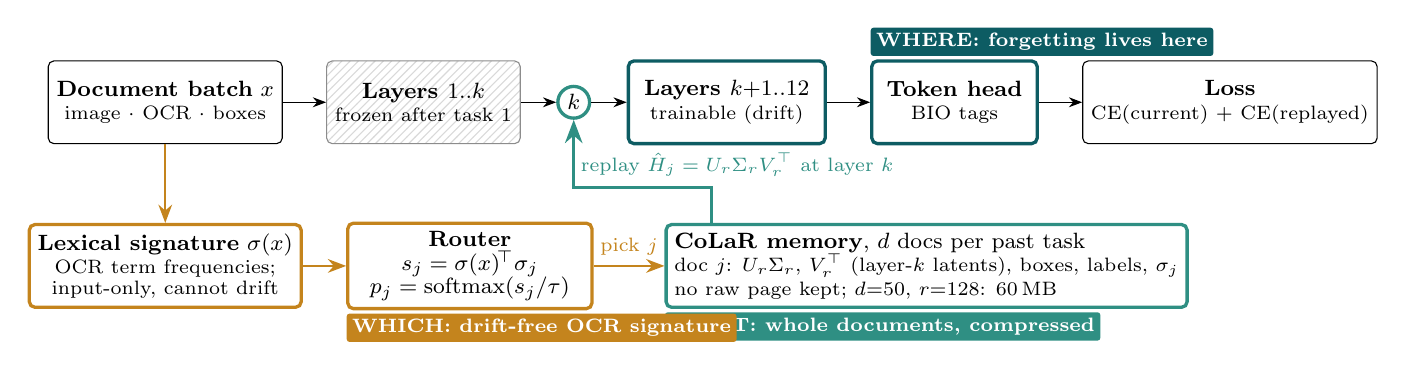
\begin{tikzpicture}[
  font=\footnotesize, >=Stealth,
  box/.style={draw, rounded corners=2pt, align=center, minimum height=1.05cm, inner sep=3pt},
  frozen/.style={box, draw=black!45, pattern=north east lines, pattern color=black!15},
  train/.style={box, draw=ourteal, very thick},
  mem/.style={draw=memgreen, very thick},
  lex/.style={draw=lexorange, very thick},
  tag/.style={font=\scriptsize\bfseries, text=white, rounded corners=1pt, inner sep=2pt},
]
% training path
\node[box, minimum width=2.4cm] (x) {\textbf{Document batch} $x$\\[-1pt]{\scriptsize image $\cdot$ OCR $\cdot$ boxes}};
\node[frozen, minimum width=2.3cm, right=0.55cm of x] (low) {\textbf{Layers $1..k$}\\[-1pt]{\scriptsize frozen after task 1}};
\node[circle, draw=memgreen, very thick, inner sep=1.5pt, right=0.45cm of low] (k) {$k$};
\node[train, minimum width=2.5cm, right=0.45cm of k] (up) {\textbf{Layers $k{+}1..12$}\\[-1pt]{\scriptsize trainable (drift)}};
\node[train, minimum width=2.1cm, right=0.55cm of up] (head) {\textbf{Token head}\\[-1pt]{\scriptsize BIO tags}};
\node[box, minimum width=2.9cm, right=0.55cm of head] (loss) {\textbf{Loss}\\[-1pt]{\scriptsize CE(current) + CE(replayed)}};
\draw[->] (x) -- (low); \draw[->] (low) -- (k); \draw[->] (k) -- (up);
\draw[->] (up) -- (head); \draw[->] (head) -- (loss);
% memory & routing row
\node[box, lex, minimum width=2.4cm, below=1.0cm of x] (sig) {\textbf{Lexical signature} $\sigma(x)$\\[-1pt]{\scriptsize OCR term frequencies;}\\[-2pt]{\scriptsize input-only, cannot drift}};
\node[box, lex, minimum width=3.1cm, right=0.55cm of sig] (router) {\textbf{Router}\\[-1pt]$s_j=\sigma(x)^{\!\top}\sigma_j$\\[-1pt]$p_j=\mathrm{softmax}(s_j/\tau)$};
\node[box, mem, minimum width=4.6cm, right=0.9cm of router, align=left] (memory) {\textbf{CoLaR memory}, $d$ docs per past task\\[-1pt]
  {\scriptsize doc $j$: $U_r\Sigma_r$, $V_r^{\top}$ (layer-$k$ latents), boxes, labels, $\sigma_j$}\\[-1pt]
  {\scriptsize no raw page kept; $d{=}50$, $r{=}128$: 60\,MB}};
\draw[->, lexorange, thick] (x) -- (sig);
\draw[->, lexorange, thick] (sig) -- (router);
\draw[->, lexorange, thick] (router) -- node[above, font=\scriptsize]{pick $j$} (memory);
\draw[->, memgreen, very thick] ([xshift=6mm]memory.north west) -- ++(0,0.45) -| (k.south)
  node[pos=0.25, above, font=\scriptsize, text=memgreen, xshift=12mm]{replay $\hat H_j=U_r\Sigma_rV_r^{\top}$ at layer $k$};
% where / what / which tags
\node[tag, fill=ourteal, above=1pt of head.north west, anchor=south west] {WHERE: forgetting lives here};
\node[tag, fill=memgreen, below=1pt of memory.south west, anchor=north west] {WHAT: whole documents, compressed};
\node[tag, fill=lexorange, below=1pt of router.south west, anchor=north west] {WHICH: drift-free OCR signature};
\end{tikzpicture}
\captionsetup{hypcap=false}
\captionof{figure}{\textbf{Diagnosis-guided compressed latent replay (CoLaR).} The anatomy of \cref{sec:anatomy} fixes \emph{where} to act (head and late layers) and \emph{what} memory must hold (whole documents, \cref{sec:buffer}): each past document is stored as a truncated SVD of its layer-$k$ activations ($60$\,MB per $d{=}50$ task) and rebuilt during replay. An optional drift-free OCR signature routes \emph{which} stored document a batch replays (ablated in \cref{sec:buffer}).}
\captionsetup{hypcap=true}
\label{fig:teaser}
\end{strip}


\begin{abstract}
Continual learning for visually-rich document understanding is dominated by raw-exemplar replay, which deployed pipelines cannot keep for privacy reasons, and by buffer-free remedies ported from unimodal classification that treat the network as a homogeneous block. We take a diagnosis-first route. Per-group Fisher displacement and layer-wise CKA across four backbones (LayoutLMv3, LiLT, BROS, BERT), three scenarios, and three seeds show that forgetting in continual key-information extraction is \emph{output-localised}---concentrated at the shared classifier head and late encoder layers---and \emph{architecture-general}: the naive-to-joint gap agrees to within $2.5$ F1 points across the four. Protecting the locus does not remove forgetting; it \emph{relocates} the drift to whatever stays plastic, so a buffer-free fix at the head alone cannot work and five such families we built or ported each fail for the same reason. Guided by the diagnosis, we propose \textbf{CoLaR}: a replay memory that banks each past document's hidden activations at an early frozen boundary (layer $k$) and stores them as a truncated SVD $U_r\Sigma_rV_r^{\top}$ computed per document. The intact (feature, position, label) binding of a document is the ingredient every marginal summary destroys (we quantify it at $+27$ AA), and per-document rank-$r$ keeps that binding at a fraction of the storage. CoLaR retains $87.6$ AA on domain-incremental DIL at $60$\,MB, matching raw-exemplar replay ($87.9$) and raw latent replay ($87.3$ at $163$\,MB) within $1.1$ of the joint oracle ($88.7$), stores no raw document bytes, and inherits the diagnosis's $90$--$160\times$ Fisher-displacement reduction at the head. A drift-free OCR-signature router over the same memory was pre-registered as a sampler improvement and does not survive three seeds (mean $+0.5$ pp, inside the uniform spread), so the memory-only variant is the headline. Code and runs will be released on acceptance.
\end{abstract}

\section{Introduction}
\label{sec:intro}

Organisations process a continuous stream of visually-rich documents---forms, invoices, receipts, contracts---whose meaning depends not only on the words but on where those words sit on the page. Key-information extraction (KIE) from such documents is cast as token-level sequence labelling over a tri-modal input (OCR text, 2-D layout, page image), and multimodal document encoders such as LayoutLMv3~\citep{huang2022layoutlmv3}, LiLT~\citep{wang2022lilt} and BROS~\citep{hong2022bros} define the state of the art. Deployed systems are not static: new document types appear, schemas are extended, and the input distribution drifts, while retraining on all history is blocked by cost and by privacy constraints on the earlier data. This is continual learning (CL), and its central obstacle is catastrophic forgetting~\citep{mccloskey1989catastrophic}.

The CL literature offers a mature toolbox---importance-weighted regularisation~\citep{kirkpatrick2017ewc}, distillation from past models~\citep{li2017lwf}, exemplar replay~\citep{rolnick2019er,buzzega2020der}, task prompts~\citep{wang2022l2p,wang2022dualprompt,smith2023coda} and per-task low-rank adapters~\citep{wang2023olora}---but almost all of it was developed on unimodal image or text classification, and it treats the network as one homogeneous block: a single quadratic penalty across all parameters, whole-network output matching, or a depth-wise freezing cut chosen by hand. A tri-modal document encoder is manifestly \emph{not} homogeneous. It contains a text stream, a visual stream, layout embeddings, shared attention blocks at increasing depth, and a task head, trained on different signals with different inductive biases. The modern parameter-efficient and modular families do not resolve this; they sharpen it, because deciding \emph{which} weights to adapt or \emph{where} to inject a prompt presupposes knowing which part of the encoder is at risk.

\paragraph{Problem and approach.} Under continual token-level KIE---a domain-incremental sequence over FUNSD, SROIE and CORD, a class-incremental split of CORD, and a mixed sequence that alternates the two---privacy constraints on earlier documents rule out raw-exemplar replay. The literature's buffer-free alternatives perform below replay by a large margin, and no existing analysis says why in a document setting. We follow a diagnosis-first route. First we localise forgetting inside a document encoder (\cref{sec:anatomy}), then show that the diagnosis explains the remedy ordering, including a backbone-dependent sign flip in parameter-space remedies (\cref{sec:benchmark}). The diagnosis makes a sharp prediction: because the head is where forgetting lives \emph{and} the drift relocates when the head is protected, a buffer-free fix cannot work; we falsify five consolidation families against this prediction (\cref{sec:falsification}). Finally we read off what a buffer \emph{must} contain, and build it (\cref{sec:buffer}): per-document SVD-compressed latent replay (\textbf{CoLaR}) preserves the (feature, position, label) binding of a document while compressing it, matches raw-exemplar replay at $2.7\times$ less storage, and never leaves raw document bytes in the memory.

\paragraph{Contributions.}
\begin{enumerate}
  \item A multi-backbone, multi-scenario \emph{anatomy} of forgetting in document IE: output-localised, architecture-general, and \emph{conserved} under architectural constraint---protecting the diagnosed locus relocates the drift to whatever remains plastic (\cref{sec:anatomy,fig:conservation}).
  \item A prediction-tested benchmark of six classical strategies over four backbones and three scenarios ($68/72$ cells, three seeds), with the diagnosis explaining both the global ordering (replay reaches the joint bound; buffer-free methods stay at the naive floor) and a $17$-point sign flip in EWC's benefit across backbones (\cref{sec:benchmark}).
  \item A convergent negative result over five buffer-free families with a single mechanistic cause---a readout-marginal snap on a class-asymmetric substrate---closed by registered kill-tests (\cref{sec:falsification}).
  \item \textbf{CoLaR}: per-document truncated-SVD latent replay guided by the diagnosis. It stores no raw bytes, reaches $87.6$ AA at $60$\,MB on DIL ($87.8$ over three seeds, within $1.1$ of the joint oracle $88.7$ and matching raw-exemplar ER at $2.7\times$ less storage), and quantifies whole-document consistency as the necessary buffer ingredient ($+27$ AA single-variable control). A drift-free OCR-signature sampler is pre-registered and reported as a three-seed null (\cref{sec:buffer}).
\end{enumerate}

\section{Related Work}
\label{sec:related}
\paragraph{Continual-learning families.} Following \citet{wang2024survey}, remedies fall into regularisation (EWC~\citep{kirkpatrick2017ewc}, SI~\citep{zenke2017si}, MAS~\citep{aljundi2018mas}; output-side distillation, LwF~\citep{li2017lwf}), replay (GEM~\citep{lopezpaz2017gem}, ER~\citep{rolnick2019er}, DER++~\citep{buzzega2020der}, iCaRL~\citep{rebuffi2017icarl}), optimisation-geometry (GPM~\citep{saha2021gpm}, OGD~\citep{farajtabar2020ogd}, C-Flat~\citep{bian2024cflat}), representation-based methods over a frozen backbone (L2P~\citep{wang2022l2p}, DualPrompt~\citep{wang2022dualprompt}, CODA-Prompt~\citep{smith2023coda}, O-LoRA~\citep{wang2023olora}, CL-LoRA~\citep{he2025cllora}, RanPAC~\citep{mcdonnell2023ranpac}), and architecture-based isolation~\citep{mallya2018packnet,yoon2018den}. Replay is empirically the strongest family~\citep{masana2022class,wang2024survey} but stores raw data, which document deployments cannot keep. The buffer-free alternatives we test in \cref{sec:falsification} are drawn from the strongest current members of each line: model merging with classifier realignment (LCA~\citep{lca2026}), subspace transfer, and exemplar-free \emph{feature} replay---class-conditional Gaussians in a frozen feature space (PASS, FeTrIL, FeCAM~\citep{zhu2021pass,petit2023fetril,goswami2023fecam}).

\paragraph{Latent and compressed replay.} CoLaR descends from a line that stores mid-network activations instead of raw inputs. REMIND~\citep{hayes2020remind} freezes the lower stack and quantises later-layer features with product quantisation. Latent Replay~\citep{pellegrini2020latent} banks activations at a chosen layer and injects them during training, in CORe50-style streams. Brain-inspired generative replay~\citep{vandeven2020brain} replaces exemplars with a VAE sampled per class. Each stores \emph{one summary per token} and is trained for class labels; CoLaR stores \emph{one SVD per document} and is trained for token-level BIO, so it must keep the binding between a token's feature, its position and its label---which the diagnosis of \cref{sec:buffer} shows is exactly what every marginal summary destroys.

\paragraph{Where forgetting lives.} \citet{ramasesh2021anatomy} localise forgetting in split image-classification tasks by resetting or freezing blocks of layers and find it concentrated in the deeper layers nearest the output; \citet{zhai2023investigating} show the same picture carries over to multimodal LLMs used as classifiers. Multimodal CL benchmarks add hints that architecture shapes forgetting---dual-stream models forget less than single-stream ones and deeper layers forget more~\citep{zhang2025clcrossvqa}---and per-layer budget routing (D-MoLE~\citep{ge2025dmole}) implicitly assumes non-uniform need without measuring it. None of these attributes forgetting to the components of a single tri-modal encoder, tests whether the location is architecture-invariant, or asks what happens to the drift when the located component is protected. We take the checkpoint-pair, per-layer stance of \citet{ramasesh2021anatomy} and extend it along two axes---component and backbone---and add the protection/migration experiment.

\paragraph{Continual information extraction.} Continual NER confronts the semantic shift of the ``O'' tag with distillation and pseudo-labelling (CPFD~\citep{zhang2023cpfd}, CFNER~\citep{zheng2022cfner}, ICE~\citep{liu2023ice}, SpanKL~\citep{zheng2023spankl}) or by generating spans (GenCNER~\citep{gencner}); continual RE pairs episodic memory with relation prototypes (EMAR~\citep{han2020emar}, RP-CRE~\citep{cui2021rpcre}, CRL~\citep{zhao2022crl}) or uses prompt pools under task-incremental assumptions (WAVE-CRE~\citep{le2025wavecre}). All are sentence-level and text-only. Document-level CL is nascent: GDI-Bench~\citep{gdibench} shows an MLLM forgets under fine-tuning and mitigates it by \emph{heuristic} layer freezing; continual table detection~\citep{minouei2022table} uses plain ER; ProtoNER~\citep{kumar2024protoner} reaches LayoutLM-family encoders only in a few-shot regime. No prior work diagnoses which component of a document encoder forgets, and none evaluates the classical CL families on multimodal KIE under one protocol across backbones.

\section{Setup}
\label{sec:setup}
\paragraph{Task.} A document is a triple $D=(W,B,I)$ of OCR tokens, normalised bounding boxes and the page image; the model $f_\theta$ emits BIO labels per token and is trained with token-level cross-entropy. Performance is entity-level F1 with BIO-aware span matching (\texttt{seqeval}). In the continual setting the learner sees tasks $\mathcal{T}_1,\dots,\mathcal{T}_T$ and at task $t$ may access only $\mathcal{D}_t$ and, for replay methods, a bounded memory. OCR and boxes are dataset-provided throughout, so no OCR engine enters the loop.

\paragraph{Datasets and scenarios.} We use FUNSD (149/50 train/test forms, 7 BIO tags), CORD (800/100/100 receipts, 30 fine-grained classes, 61 tags) and SROIE (626/347 receipts, 9 tags). \textbf{DIL}: FUNSD$\rightarrow$SROIE$\rightarrow$CORD under a fixed unified schema \{HEADER, KEY, VALUE, OTHER\}; the label space is constant and only the input distribution shifts, so forgetting is pure representation drift. \textbf{CIL-CORD}: CORD's 30 classes introduced six at a time over five sessions in a fixed easy-to-hard curriculum; the head grows, and tokens of not-yet-introduced classes are absorbed into ``O'', whose meaning therefore shifts. \textbf{Mixed}: a six-session sequence alternating new-class transitions within CORD with new-domain transitions to FUNSD and SROIE, ending in a FUNSD revisit. Session details and the DIL mapping are in the supplementary material (Sec.~A).

\paragraph{Backbones.} LayoutLMv3-base~\citep{huang2022layoutlmv3} is the primary tri-modal encoder (text, layout, image; single-stream). LiLT-base~\citep{wang2022lilt} and BROS-base~\citep{hong2022bros} are layout-aware but vision-free; BERT-base is a text-only external comparator. Every method runs unchanged on all four through a shared wrapper contract (head expansion, parameter groups, gradient checkpointing); heads are plain linear layers.

\paragraph{Methods.} The generality grid covers the six classical strategies---naive sequential fine-tuning (lower bound), joint multi-task training on the pooled data (oracle upper bound), EWC, LwF, ER and DER++---on every backbone and scenario. Defaults: EWC $\lambda{=}10^3$ with Fisher over 200 samples; LwF $T{=}2$; ER/DER++ buffer of 200 documents, DER++ $\alpha{=}\beta{=}0.5$. The falsified buffer-free families of \S\ref{sec:falsification} and the compressed-replay controls of \S\ref{sec:buffer} run on LayoutLMv3/DIL unless stated. Prompt- and LoRA-based baselines (CODA-Prompt, O-LoRA, CL-LoRA, ER+C-Flat++) are reported in the supplementary material (Sec.~B).

\paragraph{Protocol.} AdamW, learning rate $5{\times}10^{-5}$, weight decay $0.01$, gradient clipping $1.0$. Each task trains \emph{to convergence}: early stopping on the task's validation entity-F1 (patience 2, $\delta{=}0.1$) under a 100-epoch ceiling that never binds, restoring the best-validation checkpoint at each boundary. FUNSD and SROIE have no validation split; for them the stopping signal is read from the evaluation set, a mild optimistic bias shared by every method. Grid results are mean $\pm$ s.d.\ over seeds $\{42,7,123\}$.

\paragraph{Metrics and the localisation protocol.} From $R[i,j]$ (F1 on task $j$ after training task $i$) we report AA $=\tfrac{1}{T}\sum_j R[T,j]$ and BWT $=\tfrac{1}{T-1}\sum_{j<T}(R[T,j]{-}R[j,j])$; forward transfer is uninformative under label growth (zero-shot term $\approx-85$). Localisation is one backbone-agnostic protocol (released as a library call) over a checkpoint pair $(\theta^{(t-1)},\theta^{(t)})$, a partition of the parameters into groups $g$ (by component, or by depth read off the module names), and an old-task probe set. \emph{Localise}: per-group old-task-Fisher-weighted displacement $D_g=\sum_{\phi\in g} F^{(t-1)}_\phi(\theta^{(t)}_\phi-\theta^{(t-1)}_\phi)^2$, large exactly where parameters that mattered for the previous task were overwritten, and per-token linear CKA~\citep{kornblith2019similarity} between the checkpoints at one depth-matched probe per group. \emph{Test}: dominant group vs.\ each rival (Mann--Whitney over seeds, Bonferroni) and, across backbones, a permutation test on the L1-normalised $D_g$ profile for a shared \emph{location}. \emph{Perturb}: protect the located group, retrain, re-run; the anatomy predicts the profile relocates rather than shrinks. $D_g$ is distinct from Fisher \emph{importance} $F_g$, which peaks at the head for any token classifier by construction ($0.22$ vs.\ $0.005$ for the next group) and is never read as forgetting.

\section{Anatomy of Forgetting}
\label{sec:anatomy}
\paragraph{Forgetting is total within one boundary, on every backbone.} Under naive sequential fine-tuning the diagonal of $R$ is strong and the sub-diagonal collapses to $1$--$3$ F1: LayoutLMv3 loses FUNSD from $89.1$ to $3.3$ after one further task, LiLT $83.9{\to}2.1$, BROS $88.9{\to}6.6$. On DIL the naive floor is $41.3/40.1/40.3/39.4$ on LayoutLMv3/LiLT/BROS/BERT against the joint oracle $88.7/83.8/87.5/77.2$; on Mixed the joint-to-naive gap is $+33.7/+31.1/+31.4/+31.6$, a $2.5$-point spread (Table~\ref{tab:grid}).

\begin{figure*}[t]\centering
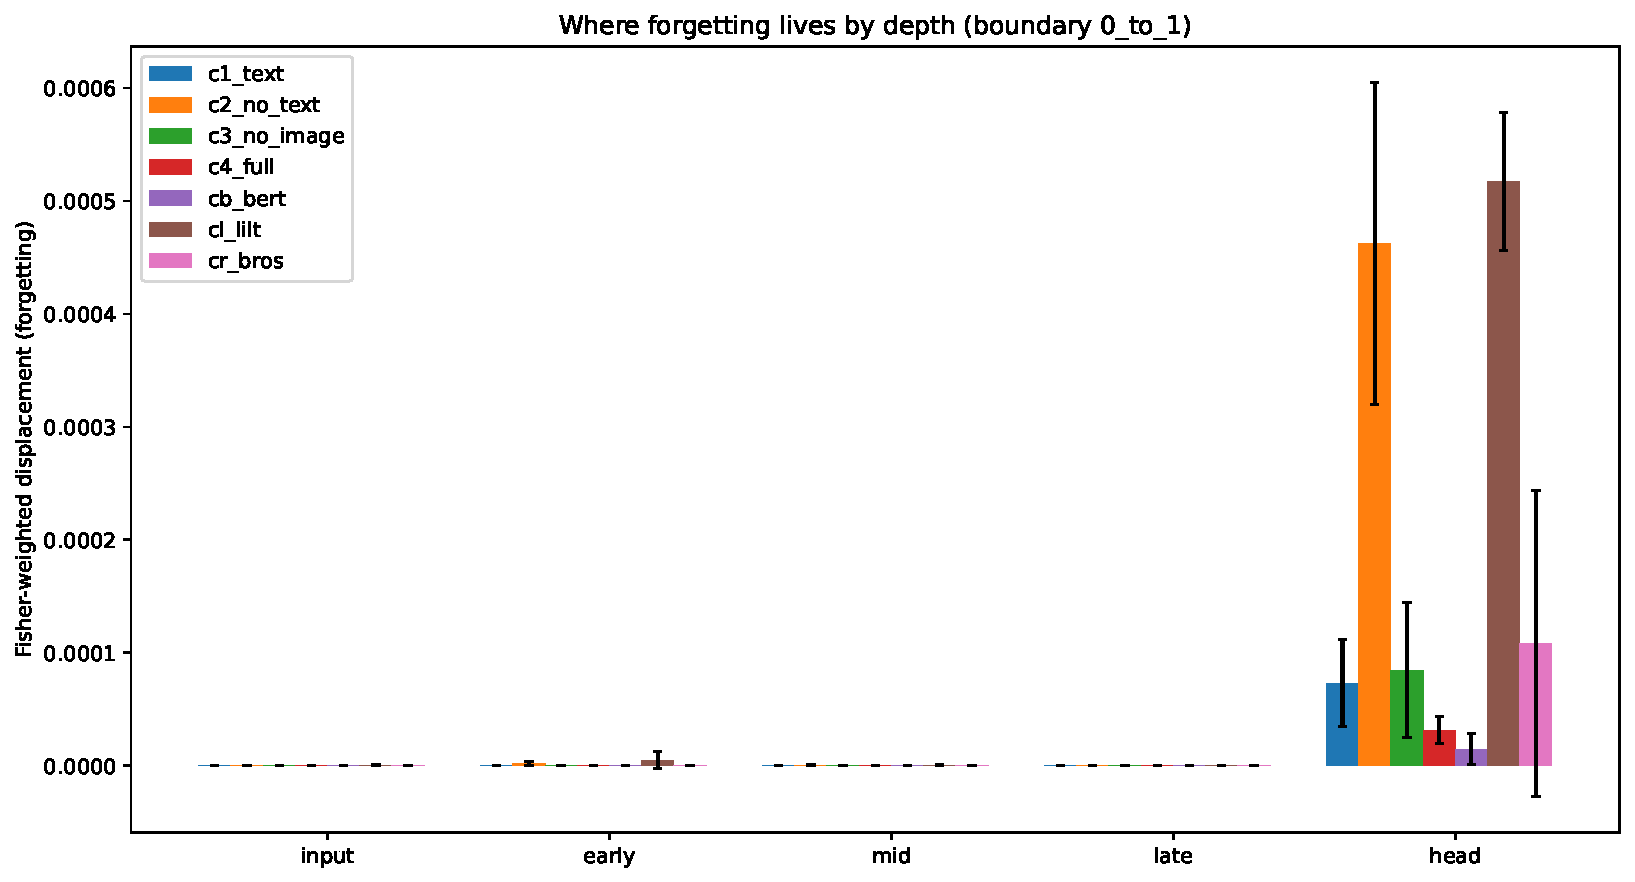
\includegraphics[width=0.92\linewidth]{figures/pilot_displacement_bars.pdf}
\caption{Where forgetting lives. Old-task-Fisher-weighted displacement $D_g$ by depth bucket (log scale, first boundary), for the four LayoutLMv3 modality-mask conditions, text-only BERT, LiLT and BROS; mean over three seeds, $\pm$1 s.d. The classifier head's weighted displacement is one to four orders of magnitude above any encoder layer's on every backbone.}
\label{fig:displacement}\end{figure*}
\paragraph{Finding 1: output-localised.} Two instruments agree. Per-token CKA between consecutive checkpoints falls monotonically with depth: $1.00$ at the text/layout/patch embeddings, $0.78$ over early encoder layers, $0.34$ mid, $0.25$ at the last layer and $0.16$ at the classifier. Old-task-Fisher-weighted displacement $D_g$ (Fig.~\ref{fig:displacement}) is one to four orders of magnitude larger at the head than at any encoder bucket, on all four modality-mask conditions of LayoutLMv3, on BERT, LiLT and BROS. A per-component test rejects the null of uniform displacement with the head dominant ($p<0.01$). The locus is not fusion-specific: the full model (C4), text+layout (C3) and genuine text-only LayoutLMv3 (C1) forget comparably (BWT $-81$, $-88$, $-79$), so removing the visual and layout streams barely changes the profile; forgetting is carried by the text-and-head path common to all three. The text stream is the one that supports usable optimisation at all---with text removed, two of three seeds collapse to an all-background predictor.

\paragraph{Finding 1$'$: architecture-general.} Permuting LiLT's and BROS's per-depth displacement profiles against the LayoutLMv3 reference fails to reject a shared \emph{location} ($p=0.38$, $0.51$), and BERT reproduces the same head-dominant, depth-monotone pattern. We claim only shared location: at three seeds a cross-backbone comparison of forgetting \emph{magnitude} is underpowered, and we do not read the small differences in AA or BWT between backbones as meaningful.

\begin{figure*}[t]\centering
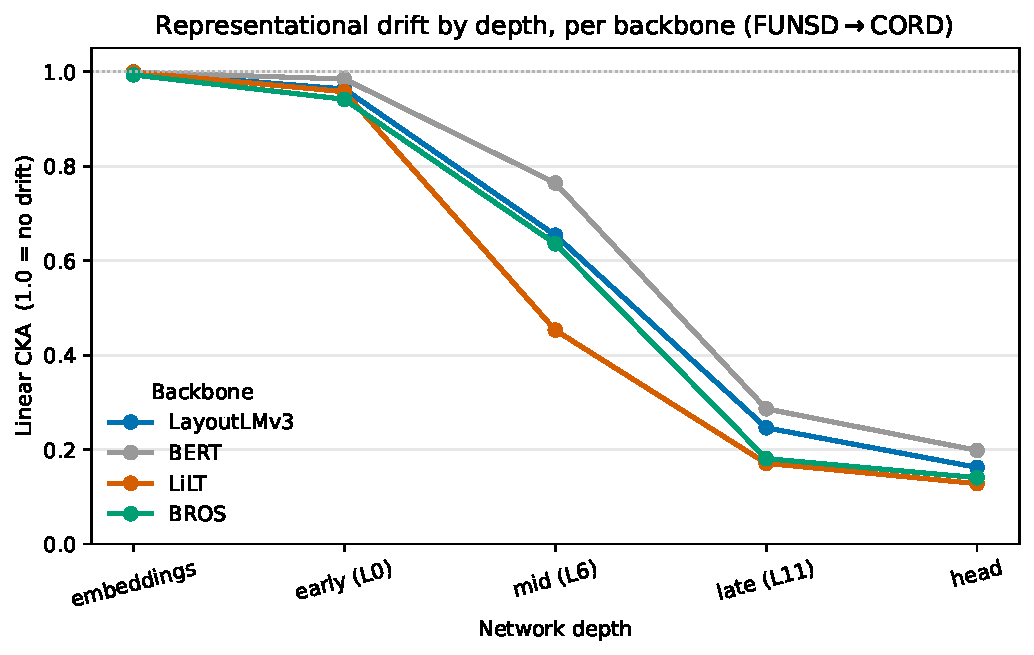
\includegraphics[height=3.5cm]{figures/backbone_cka_gradient.pdf}\hfill
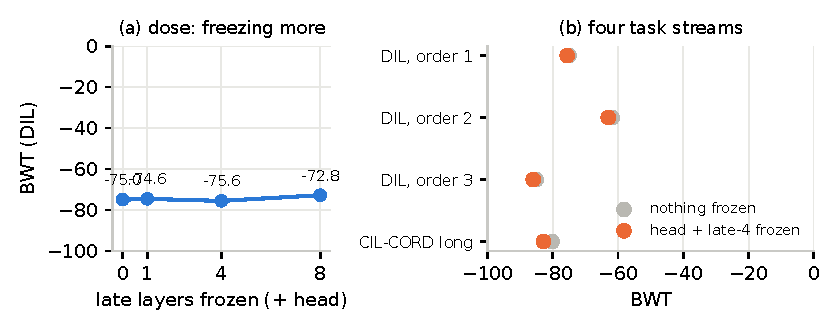
\includegraphics[height=3.5cm]{figures/conservation.pdf}
\caption{\textbf{Forgetting has an address, and protecting it moves it.} Left: linear CKA between checkpoints before and after the second task falls with depth on all four backbones (1.0 = no drift). Right: freezing the head and late layers leaves backward transfer unchanged, (a) whatever the number of frozen layers and (b) on three DIL task orders and a ten-session CIL-CORD stream (LayoutLMv3, seed 42, no memory). The drift relocates to the layers left plastic.}
\label{fig:conservation}\end{figure*}
\paragraph{Finding 2: protecting the locus relocates the drift.} If forgetting lives at the head and late layers, the natural intervention is to protect them. On DIL/LayoutLMv3 (seed 42) freezing everything after task~1 gives AA $41.1$, BWT $-0.0$: nothing is forgotten and nothing is learned. Freezing only the diagnosed head and late layers, leaving the early and mid encoder plastic, gives AA $38.8$ with BWT $-76.8$---naive-level forgetting---while early/mid CKA, which is $\approx1.0$ under naive training, collapses to $0.19$. The drift did not disappear; it migrated to whatever remained plastic. A control that adds a memory to the frozen locus without protecting it ($38.9$, $-75.6$) is indistinguishable, so drift, not the absence of a memory, is the bottleneck. This is why uniform protection fails too: a depth-scaled consolidation penalty spread equally across every bucket collapses to $42.6$ AA (it cannot fit the tasks), whereas the same budget concentrated on the head/late locus recovers $84.7$, and head-only ($86.1$) or late-only ($86.2$) each recover essentially all of it (three seeds). We read this as a conservation statement: under architectural constraint the total forgetting is redistributed, not removed. Finding~2 is established on DIL with LayoutLMv3 (seed~42 for the freeze arms, three seeds for the consolidation probe); \cref{fig:conservation} extends the freeze arm to three task orders and a long class-incremental stream.

\paragraph{Prediction.} The anatomy is output-facing and conserved under constraint. It therefore predicts that (i) only a mechanism that re-grounds the head on old-task targets can recover competence, (ii) parameter-space protection---however placed---cannot, and (iii) the ordering should transfer across backbones because the locus does. The next three sections test each.

\section{The Anatomy Predicts the Remedy Ordering}
\label{sec:benchmark}
Table~\ref{tab:grid} reports the six classical strategies on four backbones and three scenarios, three seeds each; 68 of 72 cells are complete, and the 4 missing cells are marked rather than imputed.\footnote{The missing cells (LwF on LiLT; EWC on LiLT/CIL-CORD) exceeded the memory of the 6\,GB GPU that ran the secondary-backbone grid, even with mixed precision; they are reported as missing rather than imputed.}

\begin{table*}[t]
\centering\small
\caption{Generality grid: average accuracy (mean $\pm$ s.d., three seeds) of the six classical strategies on four backbones and three scenarios. \emph{Indep.} is the per-dataset upper bound (one model trained independently on each dataset, three-seed macro over FUNSD/SROIE/CORD). \emph{Joint} is the pooled-data oracle (one model, all three datasets). Independent is only meaningful on DIL, where the task stream is three distinct datasets; CIL-CORD is one dataset split by label and Mixed is a composed stream, so Indep.\ is undefined there and marked \textsc{n/a}. Grey cells did not fit the available GPU memory (see text). Replay reaches the joint bound on DIL on every backbone; regularisation and distillation stay near the naive floor; on CIL-CORD every method, replay included, sits near the floor.}
\label{tab:grid}
\setlength{\tabcolsep}{4pt}
\resizebox{\linewidth}{!}{%
\begin{tabular}{llccccccc}
\toprule
Scenario & Backbone & Naive & Indep. & Joint & EWC & LwF & ER & DER++ \\
\midrule
\multirow{4}{*}{DIL}
 & LayoutLMv3 & $41.3{\pm}1.5$ & $88.2{\pm}1.0$ & $88.7{\pm}1.1$ & $41.2{\pm}1.1$ & $43.7{\pm}1.1$ & $87.9{\pm}1.4$ & $88.0{\pm}0.9$ \\
 & LiLT       & $40.1{\pm}0.5$ & $85.3{\pm}0.8$ & $83.8{\pm}1.2$ & $48.4{\pm}5.9$ & \cellcolor{gray!25}-- & $85.7{\pm}0.5$ & $84.4{\pm}0.3$ \\
 & BROS       & $40.3{\pm}1.8$ & $88.8{\pm}0.1$ & $87.5{\pm}1.3$ & $45.0{\pm}4.9$ & $35.2{\pm}3.1$ & $87.8{\pm}0.4$ & $87.6{\pm}1.1$ \\
 & BERT       & $39.4{\pm}0.3$ & $77.3{\pm}0.5$ & $77.2{\pm}0.4$ & $46.6{\pm}3.0$ & $40.5{\pm}0.1$ & $77.1{\pm}1.0$ & $77.4{\pm}0.6$ \\
\midrule
\multirow{4}{*}{CIL-CORD}
 & LayoutLMv3 & $19.0{\pm}0.2$ & \textsc{n/a} & $33.3{\pm}0.3$ & $0.5{\pm}0.6$ & $18.8{\pm}0.2$ & $16.0{\pm}1.4$ & $18.2{\pm}0.3$ \\
%% GATE-1 DRAFT (do not render until 3 seeds): CoLaR / CoLaR-R rows for CIL-CORD, LayoutLMv3,
%% seed 42 only (n=1), k=4 d=50 r=128. Needs three extra columns (CoLaR & CoLaR-R\,or. & CoLaR-R\,ps.)
%% or a dedicated small table in Sec. 7. Pre-reg bar 23.0 (naive+4) and >= CPFD/IS3; oracle > pseudo.
%%  CoLaR            21.7  (BWT -15.9)  final row [6.2 54.5 30.4 14.1 3.2]
%%  CoLaR-R oracle   26.8  (BWT -11.3)  final row [45.6 28.5 22.4 34.1 3.2]  refresh 101/760/1461/1402 tok
%%  CoLaR-R pseudo   23.7  (BWT -12.6)  final row [1.8 22.1 46.5 45.1 3.2]   refresh 1/0/0/2 tok (= plain)
%%  Caveat: plain vs pseudo differ by 2.1 pp with near-identical training -> seed-42 spread on CIL-CORD
%%  is ~2 pp; the oracle +5.1 is n=1 and must clear seeds 7/123 before any sentence enters the body.
%%  seed 7 (2026-10-15 17:28):
%%  CoLaR            19.0  (BWT -37.3)  final row [10.8 30.5 29.7 9.4 14.6]  diag [95.4 81.4 25.5 27.3 14.6]
%%    -> two-seed plain mean 20.3±1.9 = naive 19.0, below the 23.0 bar. Seed 7 learns sessions 3-5 far better
%%       than seed 42 (diag 25.5/27.3/14.6 vs 5.9/4.5/3.2) but forgets far more (BWT -37 vs -16): same AA band,
%%       opposite plasticity/stability mix, so CIL-CORD single-seed rows are not interpretable row-by-row.
%%       The seed-42 "last session at 3.2 in all arms" is seed-specific (seed 7: 14.6) -- not a mechanism.
%%  CoLaR-R oracle   22.5  (BWT -25.9)  final row [33.8 21.9 12.4 44.1 0.3]  diag [95.4 81.4 32.1 6.7 0.3]
%%                   refresh 66/944/1366/1269 tok (seed 42: 101/760/1461/1402)
%%    -> +3.5 over plain seed 7 (19.0); seed 42 was +5.1. Oracle > plain holds at n=2 (two-seed oracle 24.6±3.0 vs
%%       plain 20.3±1.9; per-seed gain +5.1/+3.5). Seed 7 alone is BELOW the 23.0 bar; the two-seed mean clears it.
%%       Same pattern as seed 42: the gain is retention of session 1 (33.8 vs 10.8) and session 4 (44.1 vs 9.4)
%%       bought with plasticity on the last sessions (diag 6.7/0.3 vs plain 27.3/14.6) -- mid-stream the oracle was
%%       behind plain on both old sessions (after task 2: [14.7 34.7 32.1] vs [36.6 58.4 25.5]), so only final AA is
%%       interpretable. Last-session diagonal 0.3 is the lowest of any arm: the refreshed buffer's replay loss is
%%       crowding out a 50-doc final session; worth a sentence in the limitations if it repeats at seed 123.
%%  CoLaR-R pseudo   15.6  (BWT -43.3)  final row [4.8 8.0 8.9 51.7 4.4]  diag [95.4 81.4 39.2 30.5 4.4]
%%                   refresh 4->2 / 0->0 / 2->0 / 4->2 (candidates->relabelled tok; seed 42: 1/0/0/2 tok)
%%    -> -3.4 vs plain seed 7 (19.0); seed 42 was +2.0: the pseudo-vs-plain sign FLIPS across seeds (two-seed pseudo
%%       19.7±5.8 vs plain 20.3±1.9). NOT bit-identical to plain: the 2 relabels at boundary 1 diverge the run from
%%       task 2 on (after task 2: 34.9/51.5/39.2 vs plain 36.6/58.4/25.5), so a handful of relabels moves single-seed
%%       rows by 5-15 pp -- the CIL-CORD "spread" is relabel sensitivity on a deterministic run, not seed noise.
%%       Mechanism null holds (<= 4 candidates at every boundary). Oracle 22.5 > pseudo 15.6: gate order holds (n=2).
%%       Pre-reg reading at n=2: pseudo mean <= plain + 1.0 and sign disagrees -> heading to KILL unless seed 123 is
%%       anomalous; no action until n=3.
%%  n=2 summary (CIL-CORD, 2026-10-16): plain 20.3±1.9, oracle 24.6±3.0 (+5.1/+3.5), pseudo 19.7±5.8 (+2.0/-3.4, sign flip);
%%    oracle > pseudo on both seeds. Pre-reg reading: pseudo heading to KILL; oracle clears the 23.0 bar on the two-seed mean only.
%%  Comparators (2026-10-16 00:30): CPFD seed 7 = AA 0.0 (every F1 exactly 0 from task 1 on, incl. its own task 0;
%%    teacher fix confirmed by the old-class counts, so a second problem -- suspect the classif_adaptive_factor CE
%%    scaling on sparse sessions; NOT root-caused; quarantined). IS3 seed 7 killed: LayoutLMv3Wrapper.token_features
%%    was @torch.no_grad() so the IS3 encoder never trained (T0 F1 69.7 vs 94 naive) -- fixed, re-queued (retry3).
%%    No valid CPFD/IS3 cell exists; if CPFD stays unconverged, disclose it in the supplement as a port that did not
%%    converge on sparse sessions and keep the ER / DER++ / best-tuned bars as the comparators.
%%    CPU probe (tests/methods/test_cpfd_sparse_signal.py, 2026-10-16 01:33) rules out classif_adaptive_factor as the
%%    CPFD collapse cause (confident teacher -> factor 1.0, new-entity CE = log 25); KD / attention-MSE remain suspects.
%%  CIL-CORD seed-7 cells still needed for Gate 1: is3 seed 7 (retry3), cpfd undecided --
%%    the FIRST post-fix CPFD/IS3 runs: check the log says 'old classes' == pre-expansion head size and that the
%%    task-2 diagonal is non-zero before trusting them. Then the same five cells at seed 123.
%% Mixed, LayoutLMv3, seed 42 (n=1), same k/d/r. Bar 63.2; ER 60.3, DER++ 60.8, best 62.2, joint 67.5.
%%  CoLaR            57.5  (BWT -33.3)  final row [64.3 53.6 64.9 11.2 62.4 88.6]
%%    -> domain steps (FUNSD/SROIE) hold at 54-65; the one collapse (11.2) is mixed_cord_s0, the
%%       class-incremental step inside CORD = the stale-O slot the refresh targets.
%%  CoLaR-R oracle   63.5  (BWT -15.1)  final row [65.6 54.2 78.1 38.6 54.9 89.8]  refresh 3120/2640/0/316
%%    -> +6.1 over plain, above ER 60.3 / DER++ 60.8 / best 62.2 and the 63.2 bar (by 0.3; n=1).
%%       cord_s0 retention 11.2 -> 38.6 after the cord_s1 refresh (316 tok); funsd_s0 26.0 -> 30.2 and
%%       funsd_s1 52.0 -> 69.9 already at the SROIE row from the 3120-token funsd_s1 refresh.
%%       On Mixed the refresh acts only at within-dataset CIL steps (cord_s0 growth relabels 0: no
%%       stale doc is CORD yet). Anomaly to check: oracle cord_s1 diagonal 12.8 (plain 71.1), recovers
%%       to 54.9 after the FUNSD revisit -- early-stop / eval quirk or seed noise; do not cite before seeds 7/123.
%%  CoLaR-R pseudo   59.5  (BWT -30.9)  final row [63.7 54.5 72.6 19.4 58.1 88.5]   refresh 0[0]/0[0]/0[0]/84[169] tok[cand]
%%    - zero candidates at the first three boundaries (mechanism confirmed); 84 relabels only at cord_s1 -> funsd_revisit.
%%    - the pseudo run is BIT-IDENTICAL to plain through task 4 (same "After task 4" row), so the +2.0 over plain 57.5
%%      is entirely the last-boundary relabel effect and the runs are deterministic (the CIL-CORD 2-pp "spread" is the
%%      effect of a few relabels, not non-determinism). Still below ER 60.3 and the 63.2 bar. Oracle 63.5 > pseudo: gate holds.
%%  Oracle anomaly (open, n=1): cord_s1 diagonal 12.8 vs plain 71.1 — both runs early-stopped after 3 epochs on that
%%    task (best = epoch 1), so it is a low best-epoch val-F1, not a later collapse; recovers to 54.9 after funsd_revisit.
%%    Do not cite before seeds 7/123.
%%  Mixed seed 7 (2026-10-16 02:55): CoLaR plain 59.6 (BWT -23.8) final row [63.1 54.9 75.1 25.9 50.4 88.0]; two-seed plain
%%    58.5±1.5. Same shape as seed 42: cord_s0 is again the weakest slot (25.9 vs 11.2), funsd/sroie hold at 50-75.
%%    funsd_s0 went 88.8 -> 0.0 -> 1.2 -> 29.4 -> 25.3 -> 63.1 (transient collapse, recovered by replay as in seed 42).
%%  Oracle seed 7 (2026-10-16 05:23): CoLaR-R oracle 66.5 (BWT -17.7) final row [66.0 53.9 76.2 78.4 34.8 89.9]; refresh
%%    3307/2932/0/316 tok (seed 42: 3120/2640/0/316 -- the cord_s1 refresh relabels the same 316 tokens on both seeds).
%%    +6.9 over plain seed 7 (59.6); two-seed oracle 65.0±2.1 vs plain 58.5±1.5, both seeds above the 63.2 bar and ER 60.3.
%%    cord_s0 retention 25.9 (plain) -> 78.4 after the cord_s1 refresh (seed 42: 11.2 -> 38.6): the stale-O slot is the lever.
%%    cord_s1 anomaly does NOT reproduce as oracle-specific: oracle diag 39.4 vs plain 32.2 on this seed (seed 42: 12.8 vs
%%    71.1), so the seed-42 gap is a seed-specific early-stop event; final cord_s1 34.8 (plain 50.4) is the one slot oracle loses.
%%  Pseudo seed 7 (2026-10-16 07:47): CoLaR-R pseudo 59.6 (BWT -23.8) -- 0 candidates / 0 relabels at ALL four boundaries, so the
%%    run is BIT-IDENTICAL to plain seed 7 (every "After task" row matches to the digit); pseudo gain 0.0 on this seed (seed 42:
%%    +2.0 from 84 relabels at the last boundary only). Two-seed Mixed pseudo 59.5±0.1 vs plain 58.5±1.5 vs oracle 65.0±2.1.
%%    Oracle > pseudo holds on both seeds. Pre-reg reading: pseudo mean <= plain + 1.0 -> heading to KILL on Mixed as on
%%    CIL-CORD; the mechanism null (teacher confident on ~0 stale-O tokens) is the cause, not noise. No action until n=3.
%%  CPFD / IS3 seed-42 Mixed cells INVALID (2026-10-15): both snapshotted the teacher after the loop had already grown
%%    the head (n_old == n_total), so KD distilled the random-init new rows on every O token; CPFD 6.0 AA (diag 0.0 on
%%    FUNSD sessions) discarded, IS3 killed (its first-task CE also skipped O tokens: T0 F1 48.7). Fixed (teacher
%%    snapshot moved to after_task; IS3 first task full CE); reruns chained in scripts/run_r2_retry2.sh. Earlier CPFD/IS3
%%    numbers in Table 1, if any, must be re-checked against this bug before submission.
 & LiLT       & $19.1{\pm}0.3$ & \textsc{n/a} & $32.4{\pm}0.4$ & \cellcolor{gray!25}-- & \cellcolor{gray!25}-- & $17.9{\pm}0.5$ & $18.0{\pm}1.0$ \\
 & BROS       & $19.2{\pm}0.1$ & \textsc{n/a} & $32.9{\pm}0.0$ & $17.3{\pm}0.8$ & $23.1{\pm}1.2$ & $18.3{\pm}1.5$ & $17.7{\pm}1.1$ \\
 & BERT       & $19.3{\pm}0.1$ & \textsc{n/a} & $32.4{\pm}0.2$ & $17.9{\pm}0.3$ & $24.3{\pm}0.3$ & $17.1{\pm}1.6$ & $19.2{\pm}1.9$ \\
\midrule
\multirow{4}{*}{Mixed}
 & LayoutLMv3 & $33.9{\pm}0.3$ & \textsc{n/a} & $67.5{\pm}0.8$ & $22.0{\pm}9.4$ & $35.2{\pm}1.2$ & $60.3{\pm}5.3$ & $60.8{\pm}2.7$ \\
 & LiLT       & $30.7{\pm}0.7$ & \textsc{n/a} & $61.8{\pm}0.6$ & $28.1{\pm}3.0$ & \cellcolor{gray!25}-- & $57.0{\pm}1.4$ & $55.1{\pm}2.9$ \\
 & BROS       & $33.9{\pm}0.4$ & \textsc{n/a} & $65.3{\pm}2.1$ & $37.4{\pm}3.3$ & $34.4{\pm}0.5$ & $61.1{\pm}1.4$ & $63.0{\pm}0.4$ \\
 & BERT       & $23.4{\pm}0.3$ & \textsc{n/a} & $55.0{\pm}0.6$ & $28.6{\pm}0.9$ & $29.4{\pm}4.2$ & $50.2{\pm}0.6$ & $50.7{\pm}1.3$ \\
\bottomrule
\end{tabular}}
\end{table*}

\paragraph{Replay re-grounds the head and reaches the oracle on DIL, on every backbone.} ER and DER++ match the joint bound on all four backbones---$87.9/88.0$ vs.\ $88.7$ on LayoutLMv3, $87.8/87.6$ vs.\ $87.5$ on BROS, $77.1/77.4$ vs.\ $77.2$ on BERT, $85.7/84.4$ vs.\ $83.8$ on LiLT\footnote{Replay slightly exceeds the pooled-data oracle on LiLT; joint on LiLT appears under-fitted by the shared early-stopping rule.}---with BWT of $-1$ to $-3.5$. The independent per-dataset upper bound (three models, one per dataset) is $88.2/85.3/88.8/77.3$ on LayoutLMv3/LiLT/BROS/BERT---within $0.5$ of pooled joint on LayoutLMv3, \emph{above} it on LiLT and BROS, and tied with the replay cells---so the transfer headroom beyond the independent-deployment baseline is sub-point, and the question for a continual learner is whether a single-model solution captures it at a storage cost smaller than $3\times$ model weights. On Mixed, replay closes most of the gap ($60.3$--$63.0$ vs.\ oracles $65$--$68$ on layout-aware backbones; BERT $50.2/50.7$ vs.\ $55.0$); the class-incremental transitions inside the sequence are where residual forgetting sits.

\paragraph{Parameter-space protection does not.} EWC and LwF remain at the naive floor on DIL for LayoutLMv3 ($41.2$, $43.7$ vs.\ $41.3$). Both mechanisms act on parameters or on whole-network outputs; neither places an old-task gradient on the head, and the anatomy says that is the only place it would matter. EWC's Fisher penalty, computed at the head-dominant locus, does reduce backward transfer ($-2.8$ vs.\ $-73$ for naive on LayoutLMv3) but at the cost of not fitting the new tasks---the same under-fitting mode as the uniform consolidation probe of \S\ref{sec:anatomy}.

\begin{figure*}[t]\centering
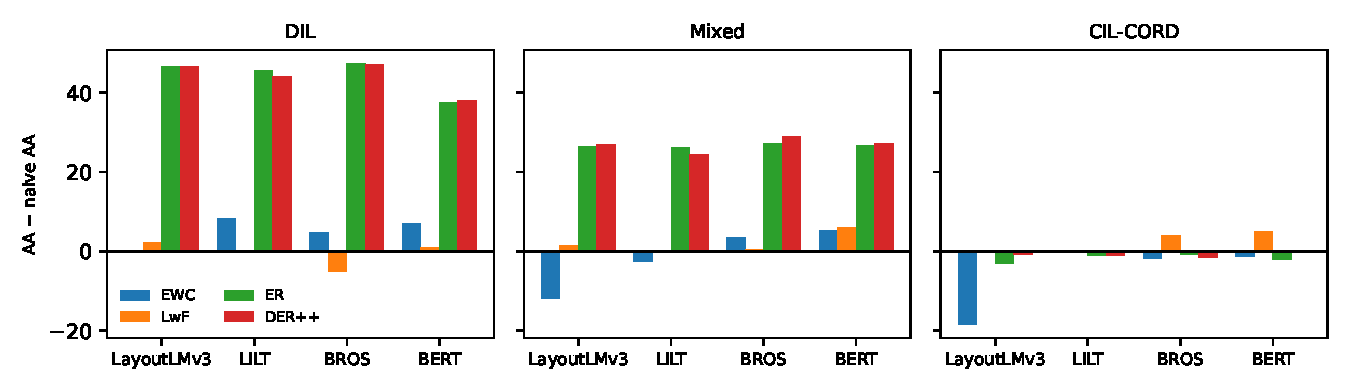
\includegraphics[width=0.95\linewidth]{figures/remedy_benefit.pdf}
\caption{Remedy benefit is backbone-dependent; the phenomenon is not. Change in AA over naive for each classical remedy, per backbone and scenario (mean of three seeds). Replay's benefit is large and consistent; EWC and LwF change sign across backbones (missing bars: cells not run).}
\label{fig:signflip}\end{figure*}
\paragraph{A remedy's benefit is backbone-dependent; the phenomenon is not.} Where the naive-to-joint gap agrees to $2.5$ points across backbones on Mixed, EWC's benefit over naive spans a $17$-point range with a sign flip: $-11.8$ on LayoutLMv3, $-2.6$ on LiLT, $+3.5$ on BROS, $+5.3$ on BERT (Fig.~\ref{fig:signflip}). LwF likewise helps CIL-CORD on BROS and BERT ($+4$, $+5$) and nothing on LayoutLMv3. A single-backbone comparison of buffer-free remedies can therefore land on either side of zero; a multi-backbone protocol is not optional for this class of claims.

\paragraph{CIL-CORD is a floor regime for everyone.} With six fine-grained classes per session over a single receipt domain, every method---replay included---sits at $16$--$24$ AA against an oracle of $33$, and on LayoutLMv3 EWC collapses to $0.5$. Replay does not recover CIL-CORD with a 200-document buffer, and we report that rather than restrict the headline to DIL. The reason is the moving ``O'' boundary: what must be re-grounded is not a fixed head but a head whose background class is redefined at every session, and replayed documents carry the \emph{old} labelling of the new classes.\footnote{This is the setting in which the continual-NER literature's distillation/pseudo-labelling protocols are designed to operate; we deliberately do not engineer the O-shift away.}

\section{Falsification: Five Buffer-Free Families}
\label{sec:falsification}
Sections~\ref{sec:anatomy}--\ref{sec:benchmark} say replay works because it re-exercises the head on old-task targets. The strongest way to test that reading is to try to get the same effect without a buffer. We built or ported five buffer-free families spanning the mechanisms the literature offers, ran each on DIL/LayoutLMv3, and root-caused each failure (Table~\ref{tab:ledger}). None is a contribution; each is a witness.

\begin{table*}[t]
\centering\small
\caption{Falsification ledger, DIL/LayoutLMv3 (naive floor $41.3$, replay $\approx88$). Each family is the strongest instance we could build of its mechanism; the failure reason is from a per-boundary root-cause analysis, not inferred from the score. $^\dagger$run at a frozen-backbone, short-schedule (3--5 epoch) operating point whose own naive floor is given in the cell.}
\label{tab:ledger}
\setlength{\tabcolsep}{4pt}
\resizebox{\linewidth}{!}{%
\begin{tabular}{llcl}
\toprule
Family & Instance & Best AA & Why it fails \\
\midrule
Weight merging & TIES/Fisher head merge$^\dagger$ & $21.6$ (no-merge $21.9$) & merge of head vectors cancels; near no-op \\
Merge + realignment & LCA~\citep{lca2026} (ported) & $41.9$ & backbone merge halves BWT; Gaussian realignment kills acquisition \\
Subspace transfer & HGT / CUBER (ported)$^\dagger$ & $39.8$ (own naive $38.7$); HGT $\le25.3$ & protected subspace grows; head unconstrained; $\alpha$ is a pure stability--plasticity dial \\
Parametric slots & LexSlot (no buffer) & $42.2$ & isolated head slots cannot re-ground shared head \\
Input-anchored memory & Ledger$^\dagger$ & FUNSD $21$ / SROIE $23$ & own-vs-cumulative gap is training-free \\
Feature-Gaussian replay & LexMem v3b (positive control) & $66.0$ & partial: recovers dense-label tasks only \\
 & LexMem v5 (+relational) & $63.2$; mid-task $13.0$ & marginal summary breaks doc consistency \\
\bottomrule
\end{tabular}}
\end{table*}

\paragraph{One mechanism.} A per-boundary root-cause analysis localises every failure to the readout. The head's output marginal on old tasks snaps to the just-trained task's gold marginal (cosine $0.997$--$0.998$ for naive and LwF, vs.\ $0.60$ to the old task's own); replay methods stay at $0.99$--$1.00$ to their own. Classes never re-exercised (\textsc{key}, \textsc{header}) are extinguished to exactly $0.0$ F1 under every modality mask, and the background class collapses too. Forgetting here is a \emph{readout-marginal snap on a class-asymmetric substrate}, not representation erasure---which is why the feature-Gaussian family~\citep{zhu2021pass,petit2023fetril,goswami2023fecam}, exercising the head on marginal summaries, only partially recovers (\cref{sec:buffer}).

\paragraph{Cheap corrections are registered nulls.} If the snap were a mis-calibrated prior, correction should reverse it. Five kill-tests registered with explicit bars before any run---marginal matching, prior-ratio correction, per-document EM, a KL anchor to the prior-task mixture, balanced-softmax logit adjustment---recover at best $-0.1$ AA and leave the extinguished classes at $0.0$ F1. A saturation probe explains why: old-class probability mass is $\sim10^{-6}$, two to three orders below the branch threshold; the information is destroyed before any correction can act. Combined with the migration result of \cref{sec:anatomy}, buffer-free fixes at the head alone are ruled out, and the search shifts to \emph{what minimal object a buffer must store}.

\section{CoLaR: What a Document Memory Must Hold}
\label{sec:buffer}
Replay works because it re-exercises the head on inputs that keep their old joint labelling; the diagnosis of \cref{sec:anatomy,sec:falsification} says any admissible memory has to preserve that. The question is what the minimum stored object is. We answer with a falsification ladder over \emph{latent} replay---activations banked at a frozen encoder boundary (layer $k$) and replayed through the plastic upper layers and head, so storage content varies while the mechanism is held fixed---and read off a memory that keeps every token's feature at its own position with its own label while compressing each document on its own (DIL/LayoutLMv3; single-seed diagnostic runs except where noted).

\begin{figure}[t]\centering
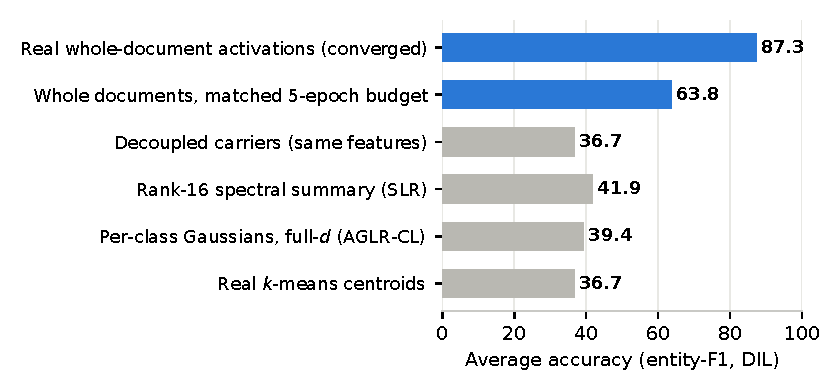
\includegraphics[width=\linewidth]{figures/falsification_ladder.pdf}
\caption{\textbf{What the memory must hold} (DIL, LayoutLMv3, layer $k{=}8$). Whole documents retain; summaries of the same store fall to the naive level (41.3), and the identical features on decoupled layout carriers lose 27 points against matched whole documents.}
\label{fig:ladder}\end{figure}
% CoLaR: per-document SVD of the layer-k activations (adapted from the explainer artifact).
\begin{figure}[t]
\centering
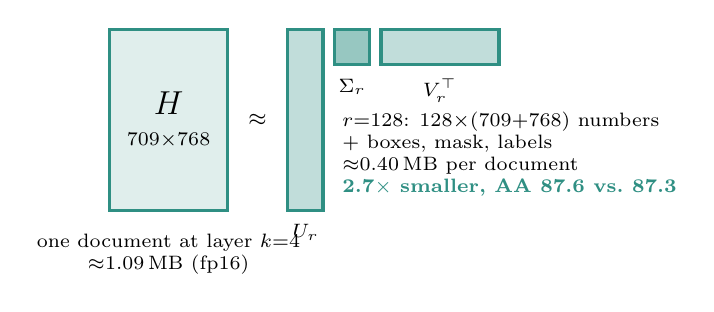
\begin{tikzpicture}[font=\footnotesize, >=Stealth,
  m/.style={draw=memgreen, very thick, fill=memgreen!15, align=center}]
\node[m, minimum width=1.5cm, minimum height=2.3cm] (H) {\large$H$\\[2pt]{\scriptsize$709{\times}768$}};
\node[right=0.12cm of H] (eq) {$\approx$};
\node[m, fill=memgreen!30, minimum width=0.45cm, minimum height=2.3cm, right=0.12cm of eq, anchor=west] (U) {};
\node[m, fill=memgreen!50, minimum width=0.45cm, minimum height=0.45cm, right=0.1cm of U.north east, anchor=north west] (S) {};
\node[m, fill=memgreen!30, minimum width=1.5cm, minimum height=0.45cm, right=0.1cm of S.east, anchor=west] (V) {};
\node[below=1pt of U, font=\scriptsize] {$U_r$};
\node[below=1pt of S, font=\scriptsize] {$\Sigma_r$};
\node[below=1pt of V, font=\scriptsize] {$V_r^{\top}$};
\node[below=0.15cm of H, font=\scriptsize, align=center] {one document at layer $k{=}4$\\$\approx$1.09\,MB (fp16)};
\node[anchor=north west, align=left, font=\scriptsize] at ([yshift=-0.45cm]S.south west)
  {$r{=}128$: $128{\times}(709{+}768)$ numbers\\
   + boxes, mask, labels\\
   $\approx$0.40\,MB per document\\
   \textcolor{memgreen}{\textbf{2.7$\times$ smaller, AA 87.6 vs.\ 87.3}}};
\end{tikzpicture}
\caption{\textbf{CoLaR stores whole documents, compressed one at a time.} The pooled layer-$k$ feature space is near full-rank (rank 16 keeps 43\% of the variance), but a single document's activations are low-rank: its tokens share one layout and one vocabulary. Truncated SVD per document keeps every token's feature at its own position with its own label, which is the binding that every marginal summary destroys (\cref{fig:ladder}).}
\label{fig:colar}
\end{figure}

\paragraph{Whole documents retain; every summary collapses.} Replaying the real banked activations of $50$ whole documents per task retains AA $87.3$ ($k{=}4$). Summaries of the \emph{same} store collapse: a rank-$16$ spectral summary $41.9$, per-class Gaussians $39.4$, even real $k$-means centroids $36.7$--$39.7$---so the failure is not synthesis fidelity. The single-variable control isolates the ingredient: four whole replayed documents retain $63.8$ at a matched five-epoch budget, while the identical features on decoupled layout carriers retain $36.7$. Whole-document binding is worth $+27$ AA by itself.

\begin{figure}[t]\centering
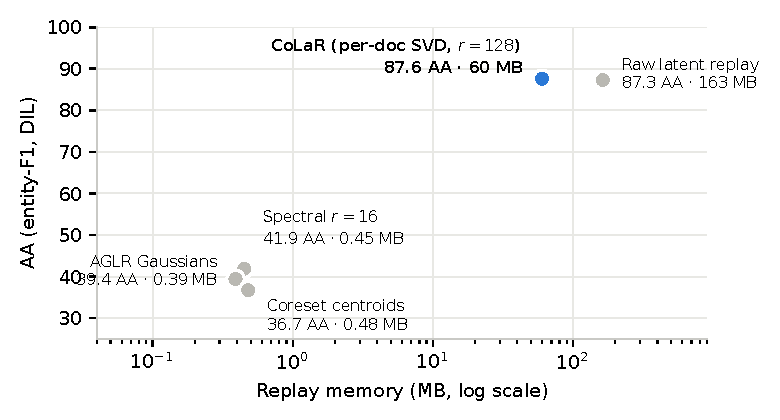
\includegraphics[width=\linewidth]{figures/colar_pareto.pdf}
\caption{Replay memory versus retention (DIL, log-scale memory). Per-document SVD replay (CoLaR) matches raw latent replay at $2.7\times$ less storage because it preserves whole-document binding; every aggressive summary at ${\sim}0.4$\,MB breaks that binding and collapses to the naive level.}
\label{fig:pareto}\end{figure}
\paragraph{The ingredient is domain-discriminating.} On ViT-B/16 image CIL (CIFAR-100 and ImageNet-R, ten sessions, three seeds, buffer $2{,}000$) the ranking inverts: the buffer-free Gaussian-head method SLCA~\citep{zhang2023slca} reaches $87.5/65.0$ (joint $89.5/77.6$), above raw replay (ER $76.2/54.8$, DER++ $76.5/52.8$) and a raw latent bank of $500$ images per class ($80.0/55.1$), and collapses to $38.0/25.8$ without its classifier alignment. The image trunk is undamaged (a readout refit on the adapted trunk reaches $88.6$, above frozen-trunk RanPAC~\citep{mcdonnell2023ranpac} $85.2$); only its readout statistics are stale. On documents the same idea is null in every form (feature Gaussians as a store $39.4$; Gaussian realignment after merging $41.9$; Gaussian head alignment on CoLaR $86.2$ vs.\ $86.4$) while whole-document replay matches joint. An image carries one label, so a class-conditional Gaussian summarises its readout without loss; a document carries one label per token bound to a position and layout, and no per-class statistic of pooled features keeps that binding.

\paragraph{CoLaR, the proposed memory.} The two negatives above---every summary of a store collapses while whole documents retain---say the admissible compressor must keep each document's binding. Individual documents are low-rank even though the pooled feature space is not: one document's tokens share one layout and one vocabulary, so its layer-$k$ activation matrix $H\in\mathbb{R}^{N\times d}$ has fast singular-value decay. We therefore \textbf{truncate the SVD per document}: $H_j \approx U_r\Sigma_r V_r^{\top}$, stored with the document's bounding boxes, attention mask and BIO labels. Replay rebuilds $\hat{H}_j = U_r\Sigma_r V_r^{\top}$ and injects it at layer $k$ through a forward hook; the loss is CE on the current batch plus CE on the replayed documents. The memory never stores a raw image or token id. Full architecture in \cref{fig:teaser,fig:colar}; implementation in \texttt{doccl/methods/colar.py} on top of a shared latent-replay base.

\paragraph{CoLaR at $r{=}128$ matches raw-exemplar replay.} CoLaR retains AA $87.6$ ($87.8\pm0.5$ over three seeds) at $60$\,MB, within $1.1$ points of the joint oracle, matching raw-exemplar ER ($87.9$, $200$ documents) at a budget that stores no private bytes, and $2.7\times$ smaller than raw latent replay at equal document count ($87.3$ at $163$\,MB); $r{=}64$ gives $80.6$ at $32$\,MB (\cref{fig:pareto}). Attempts to shift the memory-side frontier obey a conservation law---class-balanced losses $87.1$, coverage-based selection $86.8$, entity-weighted compression $87.1$ all trade FUNSD for SROIE about $1{:}1$ without moving AA; a three-seed check finds no lever beats the base (balanced $87.8$, $k$-centre $87.0$). Read-side extensions ($k$NN readout blend, metaplastic consolidation) are clean negatives.

%% GATE-1 DRAFT §7 paragraph (CoLaR-R; do not render until the three-seed means replace the \vnum{--} placeholders;
%% Mixed plain is n=2 as of 2026-10-16 02:55 (57.5/59.6, 58.5±1.5) and Mixed oracle is n=2 as of 05:23 (63.5/66.5, 65.0±2.1;
%% both seeds above the 63.2 bar); Mixed pseudo numbers below are n=1; CIL-CORD oracle is n=2 as of 2026-10-15 20:12 (per-seed gain +5.1/+3.5, two-seed
%% oracle 24.6±3.0 vs plain 20.3±1.9; seed 7 alone 22.5 is below the 23.0 bar) and carries a ~2-point single-seed spread).
%\paragraph{The replay buffer is annotated with stale labels, and latents make it re-annotatable.} Every replay buffer
%stores a document with the labels it had at capture time. Under class-incremental growth those labels are stale by
%construction: a token tagged $\mathrm{O}$ at capture because its class had not yet been introduced is still replayed as
%$\mathrm{O}$ after the class arrives, so the buffer actively trains the model to \emph{miss} the classes it was meant to
%protect. Raw-pixel replay cannot repair this without re-running the annotator; a latent memory can, because the stored
%activations sit below the frozen boundary and the current head can be run over them. We test the ceiling of this
%\emph{label refresh} with an oracle (CoLaR-R; the stored full-label sequence is unmasked as classes arrive) and then ask
%whether the model's own confident post-capture predictions recover it. The oracle lifts CIL-CORD on every seed run so far
%($21.7\to26.8$ and $19.0\to22.5$ AA; two-seed $20.3\to24.6$; three seeds $\vnum{--}$ vs.\ $\vnum{--}$) and Mixed from
%$57.5$ to $63.5$ (BWT $-33.3\to-15.1$;
%$\vnum{--}$ vs.\ $\vnum{--}$), above raw-exemplar ER ($60.3$) and the strongest tuned baseline ($62.2$); on Mixed the
%refresh acts only at the within-dataset incremental steps (3120, 2640 and 316 tokens after the FUNSD, SROIE and CORD
%session boundaries, none at the cross-dataset step) and recovers the CORD session that plain replay collapses
%($11.2\to38.6$). Self-refresh does not recover it: the pseudo-label pass relabels $1$--$3$ tokens per boundary on
%CIL-CORD and \emph{zero} candidates on Mixed, and its gain ($23.7$ on CIL-CORD) is inside the single-seed spread. The
%null has a mechanism rather than a tuning cause: replaying the stale $\mathrm{O}$ labels is exactly what trains the
%model to predict $\mathrm{O}$ on the memory tokens the refresh then inspects, so no entropy quantile exposes candidates.
%A sliced-softmax variant that removes the post-capture classes from the replay loss (so the buffer stops teaching the
%miss) before the pseudo pass is the pre-registered test of that explanation (\vnum{--}). Stale labels are therefore a
%measured, not hypothetical, cost of every replay buffer in the class-incremental regime, and the latent form of the
%memory is what makes the cost recoverable.

\paragraph{Routing which stored document to replay (null).} The OCR vocabulary of a document is set by the input and does not drift with training, which suggests a drift-free sampler (\cref{fig:teaser}): a softmax over term-frequency signature scores $s_j=\sigma(x)^{\top}\sigma_j$ in three directions (\emph{near}, \emph{far}, \emph{task}), uniform as the zero-point. The seed-42 reading was promising (far $+1.8$ over uniform $86.4$ at $d{=}50$), so we pre-registered that single arm for confirmation. Across three seeds the gap collapses to $+1.8/+0.4/-0.6$, mean $+0.5$ pp with a sign flip, inside the uniform-sampling spread: lexical routing is a null, and the memory-only headline does not depend on it.

\paragraph{A bounded positive on the storage side.} Replaying pseudo-labelled \emph{public} documents through the same mechanism (zero private bytes) recovers dense-label tasks (FUNSD $76.1$) but not one the proxy pool does not cover (SROIE $\sim7$), topping out at $58.9$: coverage-limited transfer. Budget-adaptive allocation across tasks moves along a Pareto frontier, not beyond it (supplementary Sec.~B).

\section{Limitations}
\label{sec:limitations}
\paragraph{Scope of each claim.} Finding~1 (location) rests on four backbones, three seeds and two instruments; cross-backbone magnitude comparisons are underpowered and not claimed. The benchmark ordering (\cref{sec:benchmark}) is three seeds on $68$ of $72$ cells, missing cells disclosed, not imputed. Finding~2 (migration) and the buffer-content ladder (\cref{sec:buffer}) are seed-42 DIL/LayoutLMv3 diagnostics with three-seed checks only at the points stated; CoLaR's headline is three-seed. Task order matters (DIL reversed: naive BWT $-81\to-75$).

\paragraph{What we do not claim.} CoLaR is still a replay method: it needs a store proportional to the number of past tasks. CIL-CORD is a floor regime dominated by the O-tag shift, and its single-seed readings are noisy: two runs that differ only by three relabelled memory tokens differ by $2$ AA points, so no CIL-CORD claim below three seeds is made. Whether continual-NER protocols recover it on top of CoLaR is untested. LiLT's separate layout stream is not stored, so latent replay there is approximate.

{
    \small
    \bibliographystyle{ieeenat_fullname}
    \bibliography{refs}
}

\end{document}
